% Chapter 2

\chapter{Background Research}
\label{Chapter2}

This chapter contains the information found before beginning development of the program, along with some systems that are already available and a summary on them. 

\section{Politics}
Politics is probably the biggest concern when it comes to these bot accounts. They are the reason why false information spreads so fast. This is because of the way Twitter works with its trending hashtags. These bots will tweet and retweet about important and most likely incorrect matters. They also make use of popular hashtags that basically define the topic of a tweet. This then leads to these malicious tags to become trending for everyone to see.

\subsection{2016 US Elections}
The 2016 elections in America was one of the, if not the biggest outburst of Twitter bots we have yet to see. It was found that by extrapolating some findings, roughly 19\% of 20 million election related tweets originated from bots between September and October of 2016 \cite{FM7090}. 
According to the same study it was also found that around 15\% of all accounts that were involved in election related tweets were bots. Now even though that is a lot of attention for these tweets containing false information, they will mostly only be seen by people who are already on the same side and agree. However, this doesn't rule out the affects. A study by the NBER(National Bureau of Economic Research) came to the conclusion that these bots were the cause of up to 3.23\% of the votes that went towards Donald Trump \cite{NBERw24631}. 
This tells us that even if it's just marginal, it does still affect the outcomes.
\paragraph{} The interesting part of all this is that the bots immediately went silent and disappeared as the election ended. The accounts though didn't get deleted but they simply went into hibernation waiting for their next bit of propaganda that needed to be spread. In 2017, 2000 of these bots reemerged to take part in the French and German elections as well, meaning they were run by the same people. They were discovered to make up for 1 in 5 election related tweets \cite{motherjonesbot}.

\subsection{2018 US Mid-Term Election}
Following the 2016 elections, the 2018 Mid-Terms were another prime target for Twitter bots. Before the voting took place, there were automated accounts trying to discourage people from voting. Of these, 10,000 were banned by Twitter. Even legislations were signed in an attempt to control the situation \cite{BBC001}. Interestingly, nearly two weeks after the election day, there was still activity amongst these bots which accounted for a fifth of the \#ivoted tweets \cite{ETimes001}. The numbers recorded during this recent election compared to the one in 2016 was believed to be much lower. This could either be due to the reduced number of accounts being used or it could even be that the bots are now much more sophisticated and can remain undetected as they might be able to recreate human interactions and behaviour at a higher standard.

\section{Twitter junk}
Political issues aren't the only thing being caused by these bots. A study done at the University of Iowa has shown that through the third-party applications that Twitter allows its users to utilise can be, and is often abused in malicious ways such as phishing or even just spam. Twitter themselves have a way of dealing with these toxic accounts and do most of the time eventually ban them, however this study has found that 40\% of the accounts that their algorithm detected as in some way benign were located about a month before Twitter took any action towards them \cite{IOWA001}. As this does show that there are still improvements to be made even at Twitters end in terms of detection speed, we mustn't forget that there are many other parameters we must watch out for, some unknown outside of Twitter. A Twitter spokesperson wrote: 
\begin{displayquote}
	"Research based solely on publicly available information about accounts and tweets on Twitter often cannot paint an accurate or complete picture of the steps we take to enforce our developer policies" \cite{Wired001}
\end{displayquote}

\section{Random Forest}
Random forest is a supervised learning algorithm. This means the data must be labelled, otherwise the algorithm won't know what to do with it. It's a useful algorithm, as it can be utilized for both classification and regression problems. In order to understand and implement the random forest algorithm, we first need to know about its building blocks, the decision tree.\\ 
A decision tree is made up of an ensemble of branches and leaves. The branches contain the decisions, whilst the leaves determine the label that the tree believes the data belongs to. These decisions are made based on the features that best help us determine what label the data belongs to. A major downside to decision trees is that they suffer from overfitting when they become too deep with many branches.\\ 
This is where random forest comes in. As the name implies, it combines many decision trees into a forest like object where each trees outcome is thrown together and averaged out to get one answer. However, the clever thing it manages to do is the random feature selection. Each tree takes a limited number of random features from the original total and creates its own decision tree based on that. This helps it give a much more accurate result and mostly remove the overfitting aspect of the algorithm. The other form of randomness comes from the random subset of data selected with replacement for each individual tree, also known as bagging.\\
Once the subsets are decided upon and the trees are split up we must go through the nodes and decide on how to set these rules and which features to base them on. This is done using the gini impurity equation. It's the probability of any given node that a randomly selected sample would be incorrectly labelled if it was labelled by the distribution of samples in that node \cite{DataScience001}.
The gini impurity is worked out using the following equation:
\begingroup
\fontsize{20pt}{10pt}
$$ I_{G}(n) = 1 - \sum_{i=1}^{J}(p_{i}) $$
\endgroup
The gini impurity of a node $n$ is 1 minus the sum over all the classes $J$ of the fraction of examples in each class $p_{i}$ squared \cite{DataScience001}. At nodes beyond the root the gini impurity is additionally weighted by the fraction of points from its parent node. As it is the probability of incorrect labelling, we are looking for values as small as possible here. This is repeated throughout the algorithm recursively, finding the best possible values for the best features to pick until a given depth or if there is only one class' samples remaining. 
\\
\\
%make sure layout is correct here
%\clearpage
To further help understand the algorithm it's crucial that we look at the pseudocode as that's much easier to translate into code.
\\
\begin{figure}[h]
	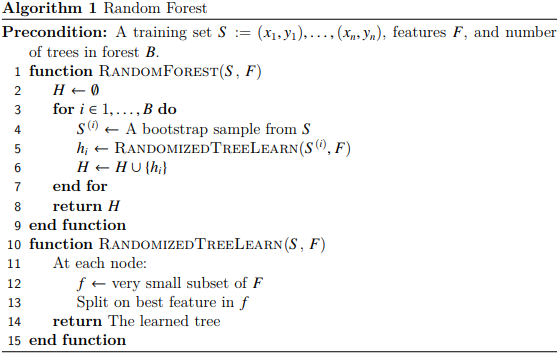
\includegraphics[width=150mm,height=100mm]{figures/pseudocode}
	\caption{Random forest pseudocode}
\end{figure}
\\

As previously mentioned, the algorithm works by creating a forest of decision trees. This means that for B number of trees we take a bootstrap or bagging sample of features from the original data and create these decision trees by splitting the nodes on the best features. Once this has been complete all the way down the trees recursively, we return the finished trees and decide based on majority vote which outcome is the most likely. 
\\
\\
\clearpage
To give a visual representation of a decision tree it would look something like the following:
\begin{figure}[h]
	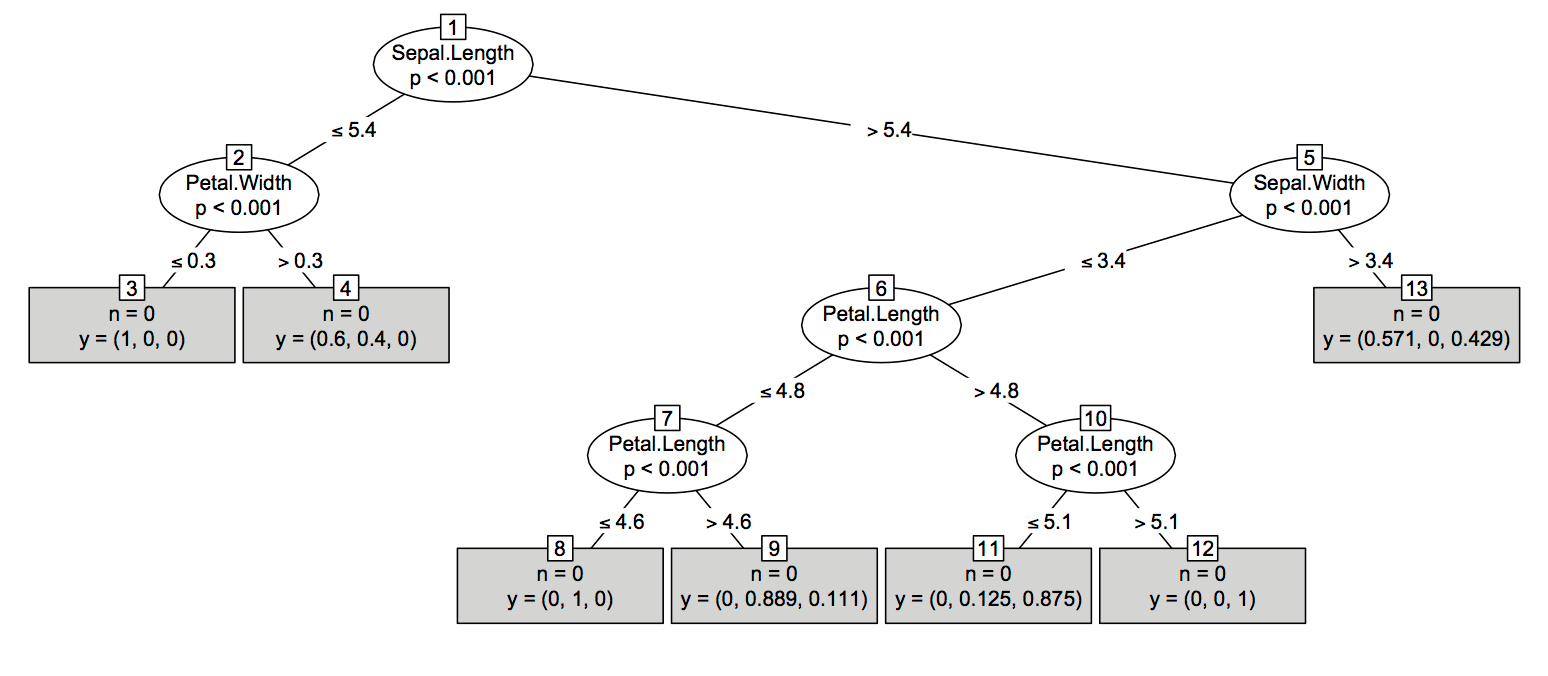
\includegraphics[width=150mm]{figures/tree}
	\caption{An example decision tree using the iris dataset}
\end{figure}
\\
Here you can see that at each node there is a condition being made. This is the 'best' feature that is decided based on the earlier mentioned gini impurity being minimised. Then based on the value of these features for a given datapoint, the algorithm will traverse down a branch of the tree all the way to a root node. This then gives us our prediction for that one decision tree within the forest. 


\section{Existing Systems}
There are a handful of algorithms or programs that have been designed to detect these bots. Most of them tend to use a machine learning algorithm as a way to classify accounts and tell them apart from each other, while others have attempted to use deep neural network architectures such as long short-term memory(LSTM).  


\subsection{Tweetbotornot}
\href{https://github.com/mkearney/tweetbotornot}{Tweetbotornot} is a package built in R that uses machine learning to classify Twitter accounts. It has two 'levels'. One for users where it uses information related to an account such as location or number of followers. The other is a tweet-level which checks for details like hashtags, mentions or capital letters out of the user's more recent 100 tweets. 
This could prove useful when testing my program to compare results as the accuracy of this library is 93.8 percent. As this is just a package created, it doesn't have any user-interface program built around it or anything like that, therefore it is unusable by anyone not knowledgable in R. 

\subsection{DeBot}
\href{https://github.com/nchavoshi/debot_api}{DeBot} is a fully functioning python API for bot detection on Twitter. It has the ability to obtain a list of bots already detected by DeBot, or just simply checking individual accounts. You can also get a list of bots which appear in the archives more than a given number of times. They can even be requested based on topics. It does however have a somewhat working built in search mechanism on its \href{https://www.cs.unm.edu/~chavoshi/debot/}{website}.
